\chapter{Prolog}
\label{sec:Prolog}
In Prolog dreht sich alles um das erstellen von Wissensbasen und deren Auswertung. Fakten und Regeln zusammen ergeben eine Wissensbasis und sind zusammen mit Anfragen die 3 Konstrukte aus denen sich diese Sprache zusammensetzt. Regeln und Fakten gehören und zu den Prädikaten. Fakten können weiterhin unterteilt werden in Funktoren und Atome. Dazu das passendes Bild. 

\begin{figure}[h]
\centering
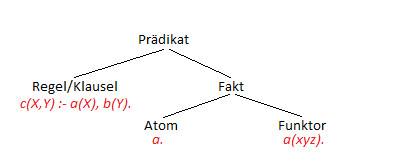
\includegraphics[width=0.5\linewidth]{mainmatter/pics/Prolog}
\caption[Prädikat Unterteilung]{Prädikat Unterteilung}
\label{fig:Prolog}
\end{figure}

\subsection{Atome}
\begin{itemize}
	\item fängt mit einem a-z
	\item bestehen aus den Zeichen a-z, A-Z, 0-9, \_
	\item Ein String in ' ' .z.B. 'Hi', auch als Name des Atoms bezeichnet. Leerzeichen sind innerhalb dieser Anführungszeichen erlaubt.
	\item Spezielle Zeichenketten sind erlaubt. Diese sind:
	\begin{enumerate}
		\item @= oder == oder ; oder :-  . Jedoch fallen ; und :- Sonderrollen zu. Mit ; fragt man nach weiteren Antworten von dem Programm und :- gehört fest zu einer Regel.
	\end{enumerate}
\end{itemize}
Hinweis: YAP und andere Prolog Interpreter erkennen 'mia' = mia. An und geben Yes aus. Jedoch '2' = 2. wird immer mit einem No konfrontiert. 
\subsection{Variablen}
\begin{itemize}
	\item Variablen beginnen mit A-Z oder \_ 
	\item bestehen aus den Zeichen a-z, A-Z, 0-9, \_
\end{itemize}\newpage
\section{Notation}
Im Nachfolgenden gibt es einen kleinen Überblick über die Notationen in Prolog.
\subsection{Und / Oder in Regeln}\qquad\\
, $\Leftrightarrow$ Und\\
; $\Leftrightarrow$ Oder
\subsection{Numerische Vergleichsoperatoren:}\qquad\\
\begin{align*}
\text{X }   &=:=  \text{  Y    numerisch gleich}\\
\text{X }  &=\backslash= \text{  Y    numerisch ungleich}\\
\text{X }   &<\text{   Y    X kleiner als Y}\\
\text{X }   &>\text{   Y    X größer als Y}\\
\text{X }  &=<\text{   Y    X kleiner gleich Y}\\
\text{X }  &>= \text{  Y    X größer gleich Y}\\
\end{align*}
!! Bei Vergleichen müssen alle Variablen belegt sein.



\subsection{Numerischer Auswertungsoperator:}\qquad\\
Ein einfaches Beispiel um X Berechnete Werte zu übergeben. \\
X is 6+3.\\
Achtung, wenn man X is Y + Z. schreibt, müssen Y und Z bereits belegt sein. Ansonsten führt dies zu einem Error. 

\subsection{Term-Vergleichsoperatoren:}\qquad\\
\begin{align*}
\text{X }   &=   \text{ Y    unifizierbar}\\
\text{X }  &\backslash=   \text{ Y    nicht unifizierbar}\\
\text{X }  &==   \text{ Y    identisch mit}\\
\text{X }  &\backslash== \text{ Y    nicht identisch mit}\\
\end{align*}




\subsection{Numerische Operatoren}

+     Addition

-     Subtraktion

*     Multiplikation

/     Division    

//    Ganzahl-Division

**    Potenz

mod   Modulo

/$\backslash$    bit-weises UND   (\& in C und C++)

$\backslash$/    bit-weises ODER  (| in C und C++)


\subsection{Typtest}\qquad\\
Dies dient zur Bestimmung des Types der einzelnen Atome.\\
atom/1 	Is the argument an atom?\\
integer/1 	Is the argument an integer?\\
float/1 	Is the argument a floating point number?\\
number/1 	Is the argument an integer or a floating point number?\\
atomic/1 	Is the argument a constant? no var, or term. \\
var/1 	Is the argument an uninstantiated variable?\\
nonvar/1 	Is the argument an instantiated variable or another term that is not an un instantiated variable? \\
Dabei gilt besonders folgendes zu beachten bei dem Test auf atom. \\

\begin{lstlisting}[language=Prolog] 
Erst instanziert dann getestet. 
?-  X  =  a,  atom(X).
X  =  a
yes

Erst getestet dann instanziert. 
?-  atom(X),  X  =  a.
no 
\end{lstlisting}
\section{Wissensbasis}\qquad\\
Als Wissensbasis bezeichnet man eine Zusammenstellung von Fakten und Regeln. Im folgenden Beispiel ist alles vorhanden. 
\begin{lstlisting}[language=Prolog] 
happy(yolanda).
listens2Music(mia).
listens2Music(yolanda):-  happy(yolanda).
playsAirGuitar(X):-  listens2Music(X). 
\end{lstlisting}
Es gibt insgesamt 2 Fakten in dieser Wissensbasis. happy(yolanda) und listen2Music(mia). Diese Fakten werden auch Funktore genannt, da diese ein Atom einklammern. Ein Reiner Fakt würde z.B. yolanda sein. \\
Die letzten Beiden Zeilen in diesem Beispiel sind Regeln. diese Zeichnen sich durch :- aus und können auch Variable gehalten werden. Die erste Regel (listens2Music(yolanda):-  happy(yolanda).) wird per Pattern Matching (siehe dazu auch das Pattern Matching in Haskell$^{\ref{sec:hpm}}$) lediglich auf die Anfrage\\ ?-listen2Music(yolanda) reagieren. Alle anderen Fälle fängt die zweite Regel ab. Hier werden die Eingaben, mit X Unifiziert$^{\ref{sec:unifikation}}$. \\
Die Regel splittet sich in einen Kopf und einen Körper auf. Alles was vor dem :- steht ist der Kopf und alles was danach steht ist der Körper. 
\section{Rekursionen}\qquad\\
Auch in Prolog gibt es Rekursionen und diese werden stark genutzt. Damit können zum Beispiel Listen durchgearbeitet werden um zu schauen, wie lange eine Liste ist. Listen können hier beliebige Datentypen enthalten und sind nicht Typisiert wie in Haskell. 
\begin{lstlisting}[language=Prolog] 
len([],0) .
len([_|T],N):-len(T,X) ,N is X + 1.

Aufruf:
?- len([1,2,3,4],X).

Ergebnis:
X = 4?
yes
\end{lstlisting}
Nehmen wir diese Rekursion einmal auseinander.\\
Die erste Zeile in diesem Beispiel ist die Abbruch Bedingung. Diese wird wahr, wenn die Liste leer ist und definiert die Länge der leeren Liste als 0. Zu dieser 0 wird jeweils durch Backtracking, dem zurück schreiten im Lösungsbaum, eine eins hinzu addiert. Dies ergibt die Länge der Liste. \\
\qquad\\
Es ist \textbf{extrem wichtig}, dass die Abbruchbedingung als erste bei einer Rekursion genannt wird. Denn Prolog arbeitet von oben nach unten. Wenn wir zuerst die Rekursion (Zeile 2) geschrieben hätten würde dies zu einem Fehler führen. \\
Beginne bei einer Rekursion immer zuerst mit der Abbruchbedingung, und stelle den rekursiven Aufruf so weit wie möglich ans Ende der rekursiven Regel.
\section{Unifikation}\label{sec:unifikation}\qquad\\
Das Ergebnis einer Unifikation ist eine Liste von Variablenersetzungen, die man vornehmen muss, um zwei Ausdrücke identisch zu machen. Diese Liste ist Zustandsfrei (für alle Zeiten gleich und unveränderlich).\\ Prolog legt im Hintergrund jede Variable nach einem bestimmten Muster an. Dieses Muster ist \_5874 Wobei die Zahlen abweichen können. 
\begin{lstlisting}[language=Prolog] 
Beispiel 1:
eats(fred,tomatoes).
eats(Whom,What) .

Beispiel 2:
likes(jane,X).
likes(X,jim).

Beispiel 3:
f(foo,L).
f(A1,A1).

Beispiel 4:
X = t(X).
\end{lstlisting}\newpage
\textbf{Lösungen:}\qquad\\
\begin{enumerate}
	\item Unifikation ist möglich da Whom = fred und What = tomatoes. Bis hier hin keine große Verwunderung.
	\item Unifikation ist \textbf{nicht} möglich da X nicht gleichzeitig zwei Werten zugeordnet werden kann.
	\item Unifikation ist möglich. Denn A1 wird mit foo unifiziert und da L auch eine Variable ist, kann diese auch mit A1 und somit mit foo unifiziert werden. 
	\item Unifikation wird endlos weiter geführt. Denn X = t(X) = t(t(X)) \dots
\end{enumerate}
\section{Resolution}
\subsection{Was ist Resolution?}\qquad\\
Resolution ist die Vorgehensweise von PROLOG bei der Lösung von Anfragen.\\
Ob eine Zielanweisung zutrifft/erfüllbar ist wird durch den Widerspruch bewiesen. 
\subsection{Wie funktioniert Resolution ?}\qquad\\
Grundvoraussetzung für eine korrekte Arbeitsweise der Resolution ist eine Wissensbasis mit vollständigen, nicht widersprüchlichen Formeln. Da das Resolutionsverfahren korrekt ist wird es immer aus einer Formelmenge einen Widerspruch ableiten wenn sich darin einer befindet.\\
Die Anfrage an eine Wissensbasis ist nichts anderes als dass eine negierte Formel in die bereits vorhandene Menge gebracht wird. Trifft die Anfrage zu, so findet die Resolution einen Widerspruch und beweist somit deren Richtigkeit.\\
Dabei benutzt die Resolution das sogenannte Ableitungsverfahren. Dieses regelt das Zusammenfassen von Klauseln und geht dabei so vor:\\
Wenn der Kopf der 1.Klausel im Körper der 2.Klausel vorkommt, so kann an dieser Stelle der Körper der 1.Klausel eingesetzt werden.\\
\qquad\\
Zur Verdeutlichung:\\
1.Klausel: A :- B,C,D\\
2.Klausel: G :- E,F,A,K\\
ergibt\\
G :- E,F,B,C,D,K\\
\qquad\\
PROLOG geht dabei von oben nach unten vor, wenn mehrere vergleichbare Formeln vorhanden sind, so wird die \grqq oberste\grqq{} genommen, bei Nichterfolg wird die nächste versucht.\\
Sind mehrere Formel durch UND verknüpft, so wird dabei von links nach rechts vorgegangen, solange eine Beantwortung möglich ist. Bei verschiedenen möglichen Antworten wird immer die zuerst gefundene ausgegeben.
\newpage
\subsection{Ein Beispiel zur Vorgehensweise}\qquad\\
Gegebene Wissensbasis:\\
legs(X,2) :- mammal(X),arms(X,2).\\
legs(X,4) :- mammal(X), arms(X,0).\\
mammal(horse).\\
arms(horse,0).\\
\qquad\\
Stellt man nun die Anfrage:\\
?- legs(horse,4).\\
\qquad\\
geht PROLOG folgendermaßen vor:\\
diese Anfrage entspricht dem Kopf der 2. Regel, wenn man  nun X mit horse "unifiziert" und den Kopf durch den Körper der Regel ersetzt erhält man folgendes\\
:- mammal(horse), arms(horse,0).\\
nun wird mammal(horse)(da es ganz links steht kommt es zuerst dran) mit dem Fakt mammal(horse). aus der Wissenbasis 'gestrichen'.\\
Ebendies passiert auch mit dem arms(horse,0) welches nach der ersten "Streichung" geblieben ist und nun gestrichen wird.\\
Übrig bleibt die leere Klausel, d.h. der Widerspruch, womit die Zielanweisung als 'wahr' bewiesen wäre. 
\section{Akkumulatoren}\qquad\\
Akkumulatoren ist eine tolle Möglichkeit Variablen hoch zählen zu lassen, während eine Liste durchgegangen wird. Hier ein kleines Beispiel zur Berechnung der Länge einer Liste. \\
\begin{lstlisting}[language=Prolog] 
acclen([],A,A).
accLen([_|T],A,L):- Anew is A + 1, accLen(T,Anew,L).

Was passiert.
?-  accLen([a,b,c],0,L).
	Call:  (6)  accLen([a,  b,  c],  0,  _G449)  ?
	Call:  (7)  _G518  is  0+1  ?
	Exit:  (7)  1  is  0+1  ?
	Call:  (7)  accLen([b,  c],  1,  _G449)  ?
	Call:  (8)  _G521  is  1+1  ?
	Exit:  (8)  2  is  1+1  ?
	Call:  (8)  accLen([c],  2,  _G449)  ?
	Call:  (9)  _G524  is  2+1  ?
	Exit:  (9)  3  is  2+1  ?
	Call:  (9)  accLen([],  3,  _G449)  ?
	Exit:  (9)  accLen([],  3,  3)  ?
	Exit:  (8)  accLen([c],  2,  3)  ?
	Exit:  (7)  accLen([b,  c],  1,  3)  ?
	Exit:  (6)  accLen([a,  b,  c],  0,  3)  ? 
\end{lstlisting}
\newpage\qquad\\
Da der Rückgabewert nicht nochmal berechnet werden muss während des Backtrackings, sondern direkt bekannt ist, sind Akkumulatoren Programme effizienter als andere. \\
Besser erkenntlich wird dies wenn man sich folgendes Beispiel anschaut und durch den Kopf gehen lässt Mit hilfe des vorherigen Beispiels. \\
\begin{lstlisting}[language=Prolog] 
accRev([H|T],A,R):-accRev(T,[H|A],R).
accRev([],A,A).
rev(L,R):-accRev(L,[],R).
\end{lstlisting}
\section{Cut}\qquad\\
Das Prädikat Cut (Symbol !) wird verwendet, um unnötiges Backtracking zu verhindern. Der Cut ist stets erfolgreich.\\
\subsection{Wirkung:}\qquad\\
Wenn Prolog bei seiner Beweissuche den Cut (!) erreicht, dann können Entscheidungen links von dem Cut nicht mehr rückgängig gemacht werde.
\subsection{Arten:}\qquad\\
Ein grüner Cut schneidet Zweige des Suchbaumes ab, die keine Lösungen enthalten.\\
Ein roter Cut schneidet Zweige des Suchbaumes ab, die Lösungen enthalten. Diesen Cut sollte man vermeiden.
\subsection{Grüner Cut:}
\begin{lstlisting}[language=Prolog] 
max(X,Y,Z) :- X =< Y, !, Z=Y.
max(X,_,X).
?- max(2,3,2).
No.
\end{lstlisting}
Es wird kein Backtracking mehr betreiben um weitere unnötige Lösungen zu finden. \\
Dies war z.B. Hilfreich um bei dem Affen Beispiel in der Vorlesung den Affen, nachdem er die Banane hatte nicht noch weiter im Raum herumlaufen zu lassen. \\
\newpage
\subsection{Roter Cut}
\begin{lstlisting}[language=Prolog] 
max(X,Y,Y) :- X =< Y, !.
max(X,_,X).
?- max(2,3,2).
Yes.
\end{lstlisting}
Hier ist die Lösung offensichtlich Falsch, jedoch ist X=<Y richtig und danach erfolgt keine Prüfung mehr, auch nicht ob Y==Y ist. Dadurch ist hier die richtige und auch weitere Lösungen abgeschnitten. Also ein Roter Cut.\\

\section{Status}\qquad\\
Hier gibt es lediglich die Möglichkeit auf die Vorlesung zu verweisen, denn dort wurden alle Status aufgezeigt, in die der Affe kommen kann. Da dies lediglich ein Funktor ist, welcher ausgegeben und zu weiteren vergleichen genutzt wird, ist es kaum Sinnvoll in diesem Dokument darauf einzugehen. 